\documentclass[11pt, a4paper, twoside]{article}   	% use "amsart" instead of "article" for AMSLaTeX format

\usepackage{geometry}                		% See geometry.pdf to learn the layout options. There are lots.
\usepackage{pdfpages}
\usepackage{caption}
\usepackage{minted}
\usepackage[german]{babel}			% this end the next are needed for german umlaute
\usepackage[utf8]{inputenc}
\usepackage{color}
\usepackage{graphicx}
\usepackage{titlesec}
\usepackage{fancyhdr}
\usepackage{lastpage}
\usepackage{hyperref}
\usepackage[autostyle=false, style=english]{csquotes}
\usepackage{mathtools}
\usepackage{tabularx}
% http://www.artofproblemsolving.com/wiki/index.php/LaTeX:Symbols#Operators
% =============================================
% Layout & Colors
% =============================================
\geometry{
   a4paper,
   total={210mm,297mm},
   left=20mm,
   right=20mm,
   top=20mm,
   bottom=30mm
 }	

\definecolor{myred}{rgb}{0.8,0,0}
\definecolor{mygreen}{rgb}{0,0.6,0}
\definecolor{mygray}{rgb}{0.5,0.5,0.5}
\definecolor{mymauve}{rgb}{0.58,0,0.82}

\setcounter{secnumdepth}{4}


% the default java directory structure and the main packages
\newcommand{\srcDirBunnies}{../src/SolutionUebung1/MetaProgramming}
\newcommand{\srcDirCounter}{../src/SolutionUebung1/Counter}
\newcommand{\imageDir}{images}
% =============================================
% Code Settings
% =============================================
\newenvironment{code}{\captionsetup{type=listing}}{}
\newmintedfile[cppSourceFile]{cpp}{
	linenos=true, 
	frame=single, 
	breaklines=true, 
	tabsize=2,
	numbersep=5pt,
	xleftmargin=10pt,
	baselinestretch=1,
	fontsize=\footnotesize
}
\newmintinline[inlineCpp]{cpp}{}
\newminted[cppSource]{cpp}{
	breaklines=true, 
	tabsize=2,
	autogobble=true,
	breakautoindent=false
}

\newcommand{\xvdash}[1]{%
  \vdash^{\mkern-10mu\scriptscriptstyle\rule[-.9ex]{0pt}{0pt}#1}%
}

% =============================================
% Page Style, Footers & Headers, Title
% =============================================
\title{Übung 3}
\author{Thomas Herzog}

\lhead{Übung 3}
\chead{}
\rhead{
\includegraphics[scale=0.10]{FHO_Logo_Students.jpg}}

\lfoot{S1610454013}
\cfoot{}
\rfoot{ \thepage / \pageref{LastPage} }
\renewcommand{\footrulewidth}{0.4pt}
% =============================================
% D O C U M E N T     C O N T E N T
% =============================================
% =============================================
% 2016.10.13: 1 
% 2016.10.14: 2
% =============================================
\pagestyle{fancy}
\begin{document}
\setlength{\headheight}{15mm}
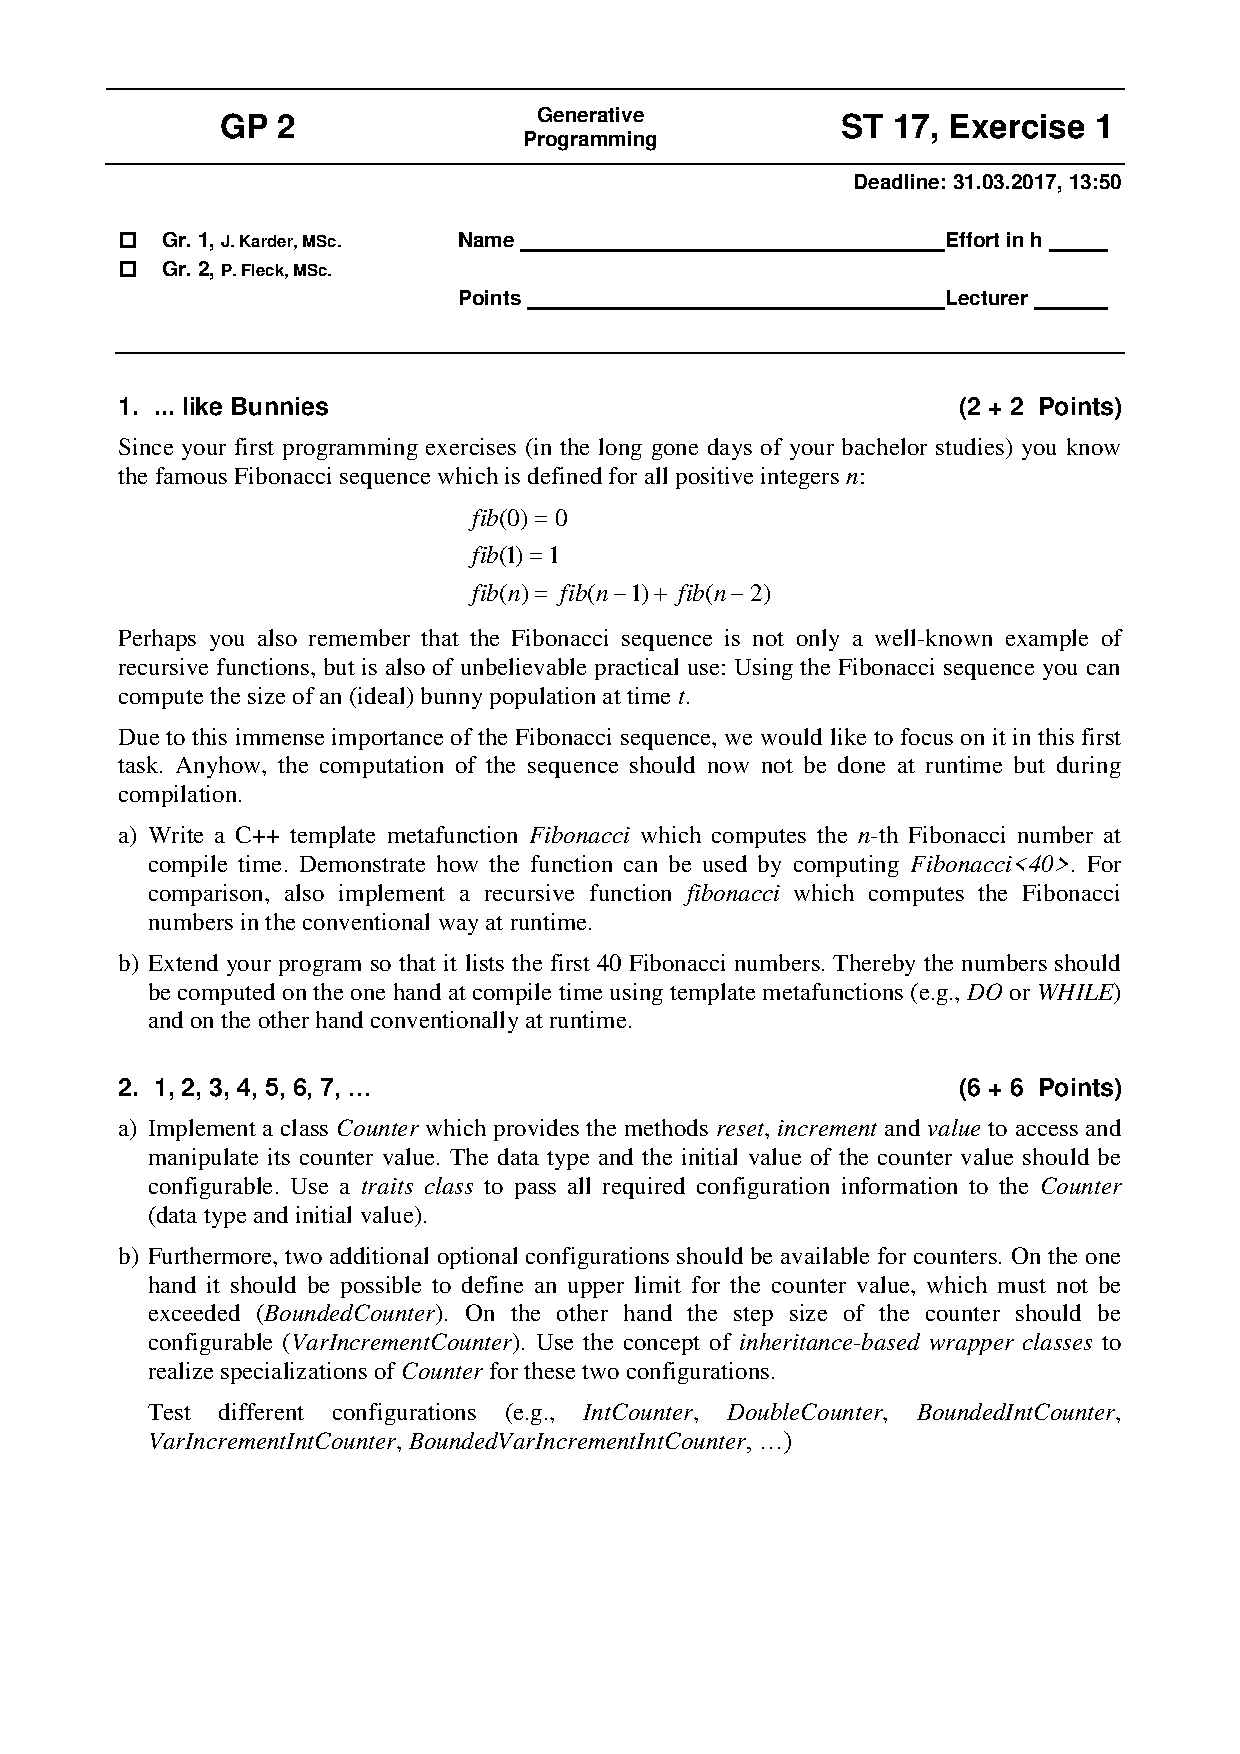
\includepdf[pages={1,2}]{GP_A01.pdf}

\section{... like Bunnies}
\subsection{Lösungsidee}
Die Implementierungen der Aufgabe \emph{like Buniies} wird in drei Dateien aufgeteilt.
\begin{itemize}
	\item fibonacci.hpp
	\item statement.hpp
	\item main.cpp
\end{itemize}
Die Berechnung der Fibonacci-Folge wird über eine rekursive Funktion implementiert, die dazu verwendet wird, die Berechnung zur Laufzeit zu durchzuführen. Es wird ein Template implementiert, welches die Fibonacci-Folge beim Kompilieren berechnet. Es werden zwei partielle Ausprägungen des Templates implementiert und zwar für die Werte 0 und 1. 0 damit die Instanziierung der Templates ein definiertes Ende hat und zusätzlich eine partielle Ausprägung für 1, da die Fibonacci-Folge wie folgt definiert ist $fib(n) = fib(n-1) + fib(n-1)$. 
\newline
\newline
Für die Berechnung der Fibonacci-Folge über \emph{DO-IF-Template-Metafunctions}, die beim Kompilieren  evaluiert werden, wird ein \emph{Template} für die Berechnung der Fibonacci-Folge implementiert, sowie ein \emph{Template} \emph{FibonacciCondition} für die Bedingung, die entscheidet, wann die Berechnung fertig ist. Um das aktuelle n im \emph{Template} zu speichern, wird folgende Anweisung verwendet \emph{enum \{ current = n \}}. Das gespeicherte n als current wird von der \emph{FibonacciCondition} benötigt, um zu entscheiden, wann die Berechnung fertig ist.
\newline
\newline
Die \emph{DO-IF-Statement Templates} werden in der Datei statement.hpp implementiert. Für das \emph{IF-Template} wird zusätzlich ein partielles \emph{Template} für den boolschen Wert \emph{false} implementiert. Das \emph{DO-Template} erwartet sich zwei Typ-Parameter \emph{Statement} und \emph{Condition}, wobei \emph{Statement} eine einfach verkettete Liste von \emph{Statements} darstellt, wobei das nächste \emph{Statement} über \emph{Statement:NEXT} verfügbar ist.

\begin{code}
	\caption{fibonacci.hpp}
	\cppSourceFile{\srcDirBunnies/fibonacci.hpp}
	\label{src:fibonacci-hhp}
\end{code}

\begin{code}
	\caption{statement.hpp}
	\cppSourceFile{\srcDirBunnies/statement.hpp}
	\label{src:statement-hhp}
\end{code}

\begin{code}
	\caption{main.cpp}
	\cppSourceFile{\srcDirBunnies/main.cpp}
	\label{src:main-cpp}
\end{code}
\ \newpage

\subsection{Tests}
\begin{figure}[h]
	\centering
	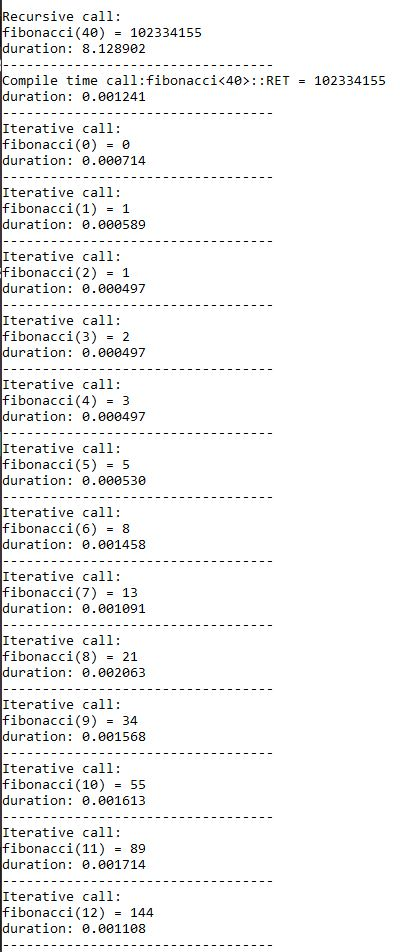
\includegraphics[scale=0.7]{\imageDir/bunnies1.JPG}
	\caption{Test Teil 1}
	\label{fig:bunnies-1}
\end{figure}
\ \newpage

\begin{figure}[h]
	\centering
	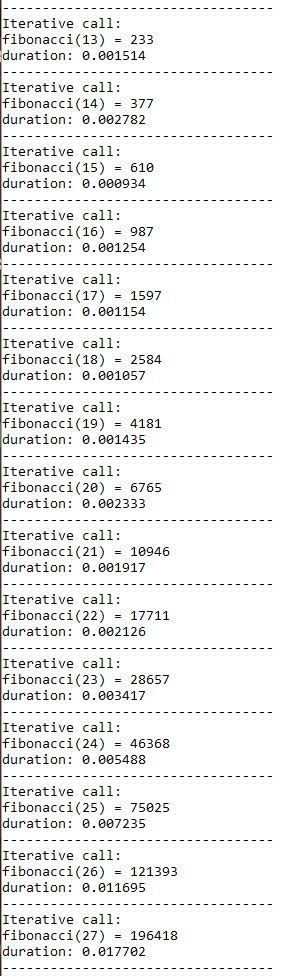
\includegraphics[scale=0.7]{\imageDir/bunnies2.JPG}
	\caption{Test Teil 2}
	\label{fig:bunnies-2}
\end{figure}
\ \newpage

\begin{figure}[h]
	\centering
	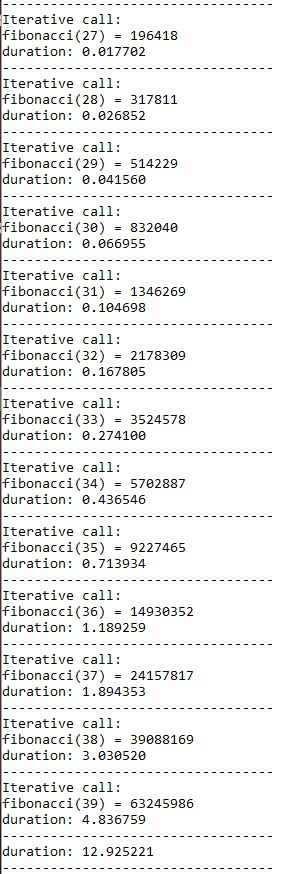
\includegraphics[scale=0.7]{\imageDir/bunnies3.JPG}
	\caption{Test Teil 3}
	\label{fig:bunnies-3}
\end{figure}
\ \newpage

\begin{figure}[h]
	\centering
	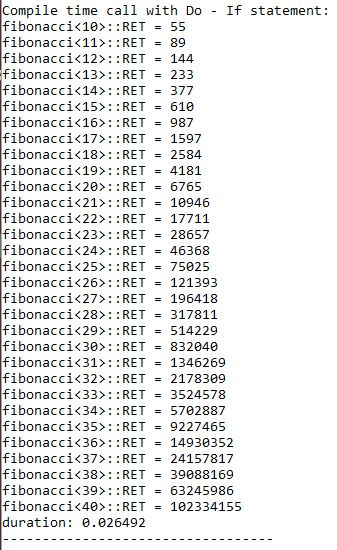
\includegraphics[scale=0.7]{\imageDir/bunnies4.JPG}
	\caption{Test Teil 4}
	\label{fig:bunnies-4}
\end{figure}
\ \newpage

\section{1, 2, 3, 4, 5, 6, ... / Counters of the Shelf}
\subsection{Lösungsidee}
Diese Aufgabenstellung wurde in den folgenden 4 Dateien implementiert:
\begin{itemize}
	\item value.hpp
	\item configuration.hpp
	\item counter.hpp
	\item boundedCounter.hpp
\end{itemize}
Für die Repräsentation der \emph{Counter}-Werte wie \emph{Inc} und \emph{Init} wird ein \emph{Template IntValue} für Integer implementiert. Für die Repräsentation von Double Werten werden für jeden verwendeten Wert \emph{Structs} implementiert, da Float und Double Zahlenwerte nicht als Template Argumente gesetzt werden dürfen, daher ist die Lösung über ein Template nicht möglich. Über eine Konstante wird der aktuelle Double Wert in das \emph{Struct} setzt.    
\newline
\newline
Es werden die 3 Konfigurationen \emph{CounterConfig}, \emph{IncCounterConfig} und \emph{BoundedCounterConfig} als \emph{Templates} implementiert, wobei die Konfiguration \emph{CounterConfig} als Basiskonfiguration fungiert, von der die anderen Konfigurationen ableiten. Die Basiskonfiguration \emph{CounterConfig} wird die Typdefinitionen \emph{ValueType}, \emph{IntValue} und \emph{IncValue} bereitstellen, die über alle Konfigurationen wieder verwendbar sind. Die Konfiguration \emph{IncCounterConf} setzt als \emph{default}-Wert für das Inkrement \emph{IntValue$<1>$}, somit ist der \emph{default Counter} immer ein \emph{(increment by one) Counter}.
\newline
\newline
Es werden die zwei \emph{Counter}-Klassen \emph{Counter} und \emph{BoundedCounter} implementiert, die über eine Konfiguration konfigurierbar sind. Es wird keine \emph{IntCounter}-Klasse \emph{(increment by one)} implementiert, da dieser \emph{IntCounter} ein \emph{Counter} mit Inkrement 1 ist und dieser \emph{IntCounter} über ein \emph{Default} für das \emph{Template}-Argument \emph{(IncValue)} der Konfiguration \emph{IncCounterConfig} realisiert werden kann. Mit diesem Ansatz kann die \emph{Counter}-Klasse wiederverwendet werden und es wird eine Klasse eingespart.
\newline
\newline
Es wird eine Konfigurator Klasse \emph{CounterConfigurator} implementiert, die je nach gesetzten \emph{Template}-Argumenten, den entsprechenden \emph{Counter} liefert. Dafür wird ein Aufzählungsdatentyp implementiert, der alle verfügbaren \emph{Counter}-Typen abbildet. \emph{Template}-Argumente, die nicht für alle \emph{Counter}-Typen benötigt werden, werden mit \emph{defaults} gesetzt, damit diese optional werden und nicht ausgeprägt werden müssen. Folgende \emph{Template}-Argumente werden auf der Konfigurator Klasse \emph{CounterConfigurator} definiert:
\begin{itemize}
	\item\emph{counterType} ist das Argument, über den der \emph{Counter}-Typ definiert wird.
	\item \emph{Init} ist das Argument, über den der Initialwert des \emph{Counters} definiert wird.
	\item \emph{Bound} ist das optionale Argument, über den der \emph{Bound} des \emph{bounded Counters} definiert wird. Als \emph{Default} wird \emph{NoBound} gesetzt.
	\item \emph{Inc} ist das optionale Argument, über den das Inkrement des \emph{Counters} definiert wird. Als \emph{Default} wird \emph{IntValue$<1>$} gesetzt.
\end{itemize}
Für die Entscheidung welcher \emph{Counter} geliefert werden muss, wird das \emph{IF-Statement} aus der Aufgabenstellung \emph{like Bunnies} verwendet. Es wird eine \emph{ELSE-IF Cascade} realisiert, die je nach gesetzter Aufzählung den entsprechenden \emph{Counter} konfiguriert und liefert.
\newline
\newline
Sollte das Inkrement beim \emph{bounded Counter} den Schwellwert überschreiten, so wird der \emph{Value} auf den zuletzt gültigen Wert gesetzt.
\ \newpage

\begin{code}
	\caption{value.hpp}
	\cppSourceFile{\srcDirCounter/value.hpp}
	\label{src:value-cpp}
\end{code}

\begin{code}
	\caption{configuration.hpp}
	\cppSourceFile{\srcDirCounter/configuration.hpp}
	\label{src:configuration-cpp}
\end{code}

\begin{code}
	\caption{counter.hpp}
	\cppSourceFile{\srcDirCounter/counter.hpp}
	\label{src:counter-cpp}
\end{code}

\begin{code}
	\caption{boundedCounter.hpp}
	\cppSourceFile{\srcDirCounter/boundedCounter.hpp}
	\label{src:bounded-counter-cpp}
\end{code}

\begin{code}
	\caption{main.hpp}
	\cppSourceFile{\srcDirCounter/main.cpp}
	\label{src:counter-main-cpp}
\end{code}
\ \newpage

\subsection{Tests}
\begin{figure}[h]
	\centering
	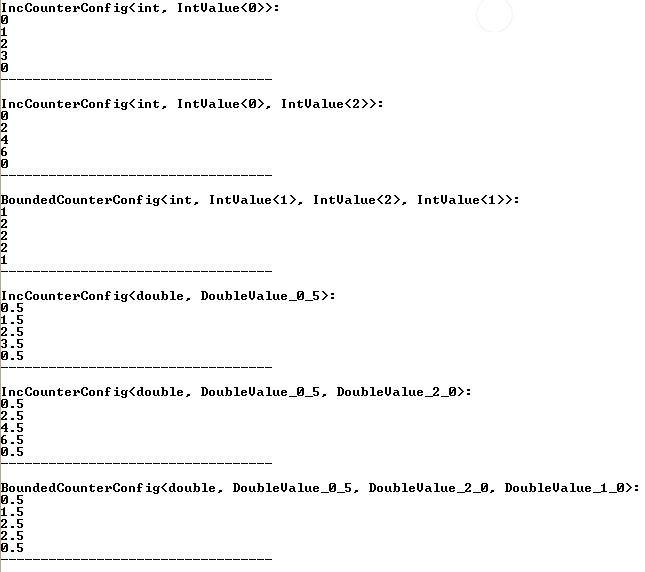
\includegraphics[scale=1]{\imageDir/counter1.JPG}
	\caption{Test Teil 1}
	\label{fig:counter-1}
\end{figure}
\ \newpage

\begin{figure}[h]
	\centering
	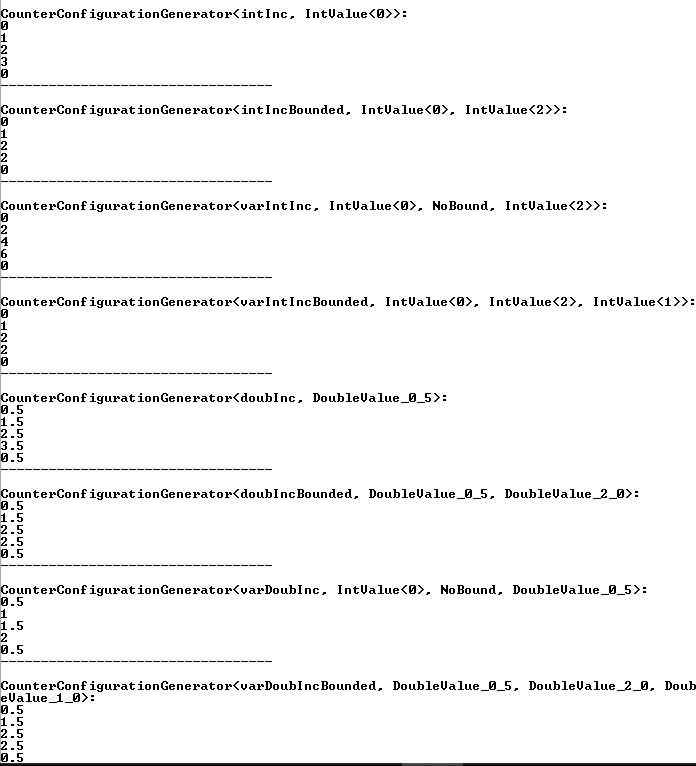
\includegraphics[scale=1]{\imageDir/counter2.JPG}
	\caption{Test Teil 2}
	\label{fig:counter-2}
\end{figure}

\end{document}